\documentclass[xcolor={dvipsnames}]{beamer}
%\documentclass[handout]{beamer} %to produce the handout

\usepackage{beamerthemeshadow}
\usepackage{graphicx}
\usepackage{textcomp}
\usepackage{xyling}
\usepackage{stmaryrd}
\usepackage{multirow}
\usepackage{pdfpages}
\usepackage[center]{caption}
\usepackage{forest}
\usepackage{caption}
\usepackage{subcaption}
\usepackage{framed}
\usepackage[vlined]{algorithm2e}

\usetikzlibrary{decorations.pathreplacing}

\definecolor{C0}{RGB}{31,119,180}
\definecolor{C1}{RGB}{255,127,14}
\definecolor{C2}{RGB}{44,192,44}
\definecolor{C3}{RGB}{214,39,40}
\definecolor{C4}{RGB}{148,103,189}

\title{An Adaptive Index for Hierarchical Database Systems}
\titlegraphic{
\includegraphics[height=.8cm]{IFIlogo.eps}}
\author{Rafael Kallis}
\institute{BSc Thesis}

\begin{document}
    \bibliographystyle{acm}
\frame{\titlepage}

%%%%%%%%%%%%%%%%%%%%%%%%%%%%%%%%%%%%%%%%%%%%%%%%%%%%%%%%%%%%%%%%%%%%%%%%%%%%%%%%%%%%%%%%%%%%%%%%%%%%%%%
%%%%%%%%%%%%%%%%%%%%%%%%%%%%%%%%%%%%%%%%%%%%%%%%%%%%%%%%%%%%%%%%%%%%%%%%%%%%%%%%%%%%%%%%%%%%%%%%%%%%%%%
%%%%%%%%%%%%%%%%%%%%%%%%%%%%%%%%%%%%%%%%%%%%%%%%%%%%%%%%%%%%%%%%%%%%%%%%%%%%%%%%%%%%%%%%%%%%%%%%%%%%%%%

\section{Introduction}
\subsection{Abstract \& Outline}
\frame{
    \begin{Large}
        The Workload-Aware Property Index (WAPI):
    \end{Large}
    
    \begin{itemize}
        \item Detects frequently updated nodes
        \item Stops pruning such volatile nodes
        \item Significantly improves update throughput
    \end{itemize}
}
\frame{
    \begin{Large}
        Unproductive Nodes are an unwanted byproduct:
    \end{Large}

    \begin{itemize}
        \item When the workload changes, volatile nodes cease to be volatile
        \item They waste space and slow down queries
        \item They do not contribute to a query match and contain no data
    \end{itemize}
}
\frame{
    \begin{Large}
        In this thesis we:
    \end{Large}

    \begin{itemize}
        \item Design and implement two solutions in order to mitigate unproductive nodes
        \item Analyze the factors impacting the production of unproductive nodes
        \item Empirically evaluate and compare our two solutions
    \end{itemize}
}
\subsection{CMS Workload}
\frame{
    \begin{large}
        A Content Management System's (CMS) workload is:
    \end{large}
    
    \begin{itemize}
        \item skewed
        \item update-heavy
        \item changing
    \end{itemize}

    %CMSs frequently use a job-queuing system that has the noted characteristics.
}
\frame{
    Skewed workload: small subset of nodes gets frequently updated
    \vspace{1cm}
    \begin{figure}
        \centering
        \begin{subfigure}{0.30\textwidth}
            \centering
            \scriptsize
            \begin{forest}
                [,circle,draw,fill=YellowOrange
                [,circle,draw,fill=YellowOrange
                [,circle,draw,fill=YellowOrange
                ]
                [,circle,draw,fill=YellowOrange
                [,circle,draw,fill=YellowOrange]
                [,phantom]
                ]
                ]
                [,circle,draw,fill=YellowOrange
                [,phantom]
                [,circle,draw,fill=YellowOrange
                [,circle,draw,fill=YellowOrange]
                [,circle,draw,fill=YellowOrange]
                ]
                ]
                ]
            \end{forest}

            No skew
        \end{subfigure}
        \begin{subfigure}{0.30\textwidth}
            \centering
            \scriptsize
            \begin{forest}
                [,circle,draw,fill=Yellow
                [,circle,draw,fill=Yellow
                [,circle,draw,fill=Yellow
                ]
                [,circle,draw,fill=Yellow
                [,circle,draw,fill=Orange]
                [,phantom]
                ]
                ]
                [,circle,draw,fill=Orange
                [,phantom]
                [,circle,draw,fill=Yellow
                [,circle,draw,fill=Red]
                [,circle,draw,fill=Orange]
                ]
                ]
                ]
            \end{forest}

            Normal skew
        \end{subfigure}
        \begin{subfigure}{0.30\textwidth}
            \centering
            \scriptsize
            \begin{forest}
                [,circle,draw,fill=Yellow
                [,circle,draw,fill=Yellow
                [,circle,draw,fill=Yellow
                ]
                [,circle,draw,fill=Yellow
                [,circle,draw,fill=Yellow]
                [,phantom]
                ]
                ]
                [,circle,draw,fill=Yellow
                [,phantom]
                [,circle,draw,fill=Yellow
                [,circle,draw,fill=Red]
                [,circle,draw,fill=Red]
                ]
                ]
                ]
            \end{forest}

            High skew
        \end{subfigure}
    \end{figure}
}
\frame{
    Changing workload: as time passes, hotspots change
    \vspace{1cm}
    \begin{figure}
        \centering
        \begin{subfigure}{0.20\textwidth}
            \centering
            \scriptsize
            \begin{forest}
                [,circle,draw,fill=Yellow
                [,circle,draw,fill=Yellow
                [,circle,draw,fill=Orange
                ]
                [,circle,draw,fill=Yellow
                [,circle,draw,fill=Red]
                [,phantom]
                ]
                ]
                [,circle,draw,fill=Yellow
                [,phantom]
                [,circle,draw,fill=Yellow
                [,circle,draw,fill=Yellow
                [,circle,draw,fill=Yellow]
                [,circle,draw,fill=Yellow]
                ]
                [,circle,draw,fill=Orange]
                ]
                ]
                ]
            \end{forest}
        \end{subfigure}
        \begin{subfigure}{0.10\textwidth}
            \centering
            $\longrightarrow$
        \end{subfigure}
        \begin{subfigure}{0.20\textwidth}
            \centering
            \scriptsize
            \begin{forest}
                [,circle,draw,fill=Yellow
                [,circle,draw,fill=Yellow
                [,circle,draw,fill=Yellow
                ]
                [,circle,draw,fill=Yellow
                [,circle,draw,fill=Yellow]
                [,phantom]
                ]
                ]
                [,circle,draw,fill=Orange
                [,phantom]
                [,circle,draw,fill=Yellow
                [,circle,draw,fill=Yellow
                [,circle,draw,fill=Orange]
                [,circle,draw,fill=Red]
                ]
                [,circle,draw,fill=Orange]
                ]
                ]
                ]
            \end{forest}
        \end{subfigure}
        \begin{subfigure}{0.10\textwidth}
            \centering
            $\longrightarrow$
        \end{subfigure}
        \begin{subfigure}{0.20\textwidth}
            \centering
            \scriptsize
            \begin{forest}
                [,circle,draw,fill=Yellow
                [,circle,draw,fill=Yellow
                [,circle,draw,fill=Orange
                ]
                [,circle,draw,fill=Yellow
                [,circle,draw,fill=Yellow]
                [,phantom]
                ]
                ]
                [,circle,draw,fill=Yellow
                [,phantom]
                [,circle,draw,fill=Yellow
                [,circle,draw,fill=Red
                [,circle,draw,fill=Orange]
                [,circle,draw,fill=Yellow]
                ]
                [,circle,draw,fill=Yellow]
                ]
                ]
                ]
            \end{forest}
        \end{subfigure}
    \end{figure}
}
\frame{
    \large
    CMSs usually use a job-queuing system that has the noted characteristics
}
\subsection{Workload-Aware Property Index}
\frame{
    \centering
    \Large
   Workload-Aware Property Index 
}
\frame{
    \frametitle{Hierarchical Database with WAPI}
    \vspace{-5mm}
    \begin{figure}[t]
        \centering
        \scriptsize
        \begin{forest}
            [
            [$\lambda:i$
            [$\lambda:\text{pub}$
            [$\lambda:\text{now}$
            [$\lambda:a$
            [$\lambda:b$
            [$\lambda:d$ \\ $\text{pub}:\text{now}$, align=center, base=bottom, name=i_node] {
                \draw[<-,gray] (.north west)--++(-5em,1em)
                node[anchor=east]{\textit{Matching Node}};
            }
            ]
            [,phantom]
            ]
            ]
            ]
            ] {
                \draw[<-,gray] (.south west)--++(-5em, -1em)
                node[anchor=east]{\textit{Index Subtree Root}};
            }
            [$\lambda:a$
            [$\lambda:b$
            [$\lambda:d$ \\ $\text{pub}:\text{now}$, align=center, base=bottom, name=c_node]
            ]
            [$\lambda:c$
            [$\lambda:e$]
            ]
            ] {
                \draw[<-,gray] (.south east)--++(5em, -1em)
                node[anchor=west]{\textit{Content Subtree Root}};
            }
            ]
            \draw[->,dotted] (i_node) to[out=east, in=south] node[gray,midway,right]{\textit{corresponding content node}} (c_node);
        \end{forest}
    \end{figure}
}
\frame{
    We mostly executes content-and-structure (CAS) queries~\cite{CM15}.
    We denote node $n$'s property $k$ as $n[k]$ and node $n$'s descendants as
    $desc(n)$.

    \begin{definition}[CAS Query]
        Given node $m$, property $k$ and value $v$, a CAS query
        $Q(k,v,m)$ returns all descendants of $m$ which have $k$ set to $v$, i.e.,
        $$ Q(k,v,m) = \{ n | n \in desc(m) \land n[k] = v\} $$
        \label{def:cas-query}
    \end{definition}
}
\frame{
    Volatility is the measure which is used by the WAPI in order to distinguish
    whether to remove a node or not from the index.
    Wellenzohn et al.~\cite{KW17} propose to look at the recent transactional
    workload to check whether a node $n$ is volatile.
}
\frame{
    \begin{definition}[Volatility Count]
        The volatility count $vol(n)$ of index node $n$ on database instance $O_i$, is the number of
        times node $n$ was added or removed from snapshots contained in a Sliding
        Window of Length $L$ over history $H_i$, i.e.,
        \vspace{3mm}
        \begin{align*}
            vol(n) = | \{ G^b | G^b \in H_i \land t(G^b) \in [t_n-L+1, t_n] \land \exists G^a[ \\
                \qquad G^a = pre(G^b) \land ([n^a \notin N(G^a) \land n^b \in N(G^b)]\lor \\
            \qquad [n^a \in N(G^a) \land n^b \notin N(G^b)] )]\} |
        \end{align*}
    \end{definition}
}
\frame{
    \begin{definition}[Volatile Node]
        Index node $n$ is volatile iff $n$'s volatility count is greater or equal than 
        the volatility threshold $\tau$, i.e.,
        \vspace{3mm}
        $$ volatile(n) \iff vol(n) \geq \tau $$
    \end{definition}
}
\frame{
    \frametitle{Index nodes becoming volatile}
    \begin{figure}
        \vspace{-1cm}
        \begin{large}
            $$ G^0 \xrightarrow{\quad T_1 \quad} G^1 \xrightarrow{\quad T_2 \quad} G^2 $$
        \end{large}
        \begin{subfigure}{0.3\textwidth}
            \centering \tiny{
                \begin{framed}
                    \begin{forest}
                        [
                        [$\lambda$:$i$
                        [,phantom]
                        ]
                        [,phantom]
                        [,phantom]
                        [$\lambda$:$a$
                        [$\lambda$:$b$
                        [$\lambda$:$d$]
                        ] 
                        [,phantom]
                        [$\lambda$:$c$
                        [$\lambda$:$e$]
                        ]
                        ]
                        ]
                    \end{forest}

                    \vspace{21mm}
                \end{framed}
                } \footnotesize{ Snapshot $G^0$

            $t(G^0) = t$ }
        \end{subfigure}
        \begin{subfigure}{0.3\textwidth}
            \centering \tiny{
                \begin{framed}
                    \begin{forest}
                        [
                        [$\lambda$:$i$
                        [$\lambda$:pub, color=RoyalBlue
                        [$\lambda$:now, color=RoyalBlue
                        [$\lambda$:$a$, color=RoyalBlue
                        [$\lambda$:$b$, color=RoyalBlue
                        [$\lambda$:$d$ \\ pub:now, color=RoyalBlue, align=center, base=bottom]
                        ]
                        [,phantom]
                        ]
                        ]
                        ]
                        ]
                        [$\lambda$:$a$
                        [$\lambda$:$b$
                        [$\lambda$:$d$ \\ pub:now, align=center, base=bottom]
                        ]
                        [$\lambda$:$c$
                        [$\lambda$:$e$]
                        ]
                        ]
                        ]
                    \end{forest}
                \end{framed}
                } \footnotesize{ Snapshot $G^1$

            $t(G^1) = t+1$ }
        \end{subfigure}
        \begin{subfigure}{0.3\textwidth}
            \centering \tiny{
                \begin{framed}
                    \begin{forest}
                        [
                        [$\lambda$:$i$
                        [$\lambda$:pub, color=RoyalBlue
                        [$\lambda$:now, color=RoyalBlue
                        [$\lambda$:$a$, color=RoyalBlue
                        [$\lambda$:$b$, color=RoyalBlue
                        [$\lambda$:$d$, color=RoyalBlue]
                        ]
                        [,phantom]
                        [,phantom]
                        ]
                        ]
                        ]
                        ]
                        [$\lambda$:$a$
                        [$\lambda$:$b$
                        [$\lambda$:$d$]
                        ]
                        [,phantom]
                        [$\lambda$:$c$
                        [$\lambda$:$e$]
                        ]
                        ]
                        ]
                    \end{forest}

                    \vspace{3mm}
                \end{framed}
                } \footnotesize{ Snapshot $G^2$

            $t(G^2) = t+2$ }
        \end{subfigure}
    \end{figure}
    \footnotesize
    $\tau = 1, L = 2$
}
\section{Unproductive Nodes}
\subsection{Introduction}
\frame{
    \centering
    \Large
    Unproductive Nodes
}
\frame{
    \begin{itemize}
        \item When nodes are volatile, their volatility count has to be at least $\tau$
        \item Time passes and the database workload changes
        \item Insertions and deletions that increased the volatility count drop out of the sliding window
        \item If the volatility count drops below threshold $\tau$, the node ceases to be volatile
        \item If the same holds for the node's descendants, we call the node and its descendants unproductive
    \end{itemize}
}
\frame{
    \frametitle{Index nodes becoming unproductive}
    \begin{figure}
        \vspace{-1cm}
        \begin{large}
            $$ G^1 \xrightarrow{\quad T_2 \quad} G^2
            \xrightarrow{\quad T_3 \quad} G^3  $$
        \end{large}
        \begin{subfigure}{0.3\textwidth}
            \centering \tiny{
                \begin{framed}
                    \begin{forest}
                        [
                        [$\lambda$:$i$
                        [$\lambda$:pub, color=RoyalBlue
                        [$\lambda$:now, color=RoyalBlue
                        [$\lambda$:$a$, color=RoyalBlue
                        [$\lambda$:$b$, color=RoyalBlue
                        [$\lambda$:$d$ \\ pub:now, color=RoyalBlue, align=center, base=bottom]
                        ]
                        [,phantom]
                        ]
                        ]
                        ]
                        ]
                        [$\lambda$:$a$
                        [$\lambda$:$b$
                        [$\lambda$:$d$ \\ pub:now, align=center, base=bottom]
                        ]
                        [$\lambda$:$c$
                        [$\lambda$:$e$]
                        ]
                        ]
                        ]
                    \end{forest}
                \end{framed}
                } \footnotesize{ Snapshot $G^1$

            $t(G^1) = t+1$ }
        \end{subfigure}
        \begin{subfigure}{0.3\textwidth}
            \centering \tiny{
                \begin{framed}
                    \begin{forest}
                        [
                        [$\lambda$:$i$
                        [$\lambda$:pub, color=RoyalBlue
                        [$\lambda$:now, color=RoyalBlue
                        [$\lambda$:$a$, color=RoyalBlue
                        [$\lambda$:$b$, color=RoyalBlue
                        [$\lambda$:$d$, color=RoyalBlue]
                        ]
                        [,phantom]
                        [,phantom]
                        ]
                        ]
                        ]
                        ]
                        [$\lambda$:$a$
                        [$\lambda$:$b$
                        [$\lambda$:$d$]
                        ]
                        [,phantom]
                        [$\lambda$:$c$
                        [$\lambda$:$e$]
                        ]
                        ]
                        ]
                    \end{forest}

                    \vspace{3mm}
                \end{framed}
                } \footnotesize{ Snapshot $G^2$

            $t(G^2) = t+2$ }
        \end{subfigure}
        \begin{subfigure}{0.3\textwidth}
            \centering \tiny{
                \begin{framed}
                    \begin{forest}
                        [
                        [$\lambda$:$i$
                        [$\lambda$:pub
                        [$\lambda$:now
                        [$\lambda$:$a$
                        [$\lambda$:$b$, color=Orange
                        [$\lambda$:$d$, color=Orange]
                        ]
                        [$\lambda$:$c$, color=RoyalBlue
                        [$\lambda$:$e$ \\ pub:now, color=RoyalBlue, align=center, base=bottom]
                        ]
                        ]
                        ]
                        ]
                        ]
                        [,phantom]
                        [$\lambda$:$a$
                        [$\lambda$:$b$
                        [$\lambda$:$d$]
                        ]
                        [$\lambda$:$c$
                        [$\lambda$:$e$ \\ pub:now, align=center, base=bottom]
                        ]
                        ]
                        ]
                    \end{forest}
                \end{framed}
                } \footnotesize{ Snapshot $G^3$

            $t(G^3) = t+3$ }
        \end{subfigure}
    \end{figure}
    \footnotesize
    $\tau = 1, L = 2$
}
\frame{
    Variables impacting unproductive node production rate:
    \begin{itemize}
        \item Volatility threshold $\tau$
        \item Sliding window length $L$
        \item Workload skew $s$
        \item Update tx per second
    \end{itemize}
}
\frame{
    Unproductive index node cleaning, we propose:
    \begin{itemize}
        \item Periodic Garbage Collection (GC)
        \item Query-Time Pruning (QTP)
    \end{itemize}
}
\subsection{Periodic Garbage Collection}
\frame{
    \centering
    \large
    Periodic Garbage Collection (GC)
}
\frame{
    \frametitle{Periodic GC}
    Main idea:

    \begin{itemize}
        \item Background process
        \item Periodically traverse index subtree
        \item Prune any visited unproductive node
    \end{itemize}
}
\frame{
    \frametitle{Periodic GC}
    \begin{algorithm}[H]
        \TitleOfAlgo{GarbageCollect}
        \DontPrintSemicolon
        \For{node $n \in desc(\texttt{/i})$ in postorder tree walk}{
            \If{$chd(n) = \emptyset \land \neg matching(n) \land \neg volatile(n)$}{
                delete node $n$\;
            }
        }
    \end{algorithm}
}
\frame{
    \frametitle{Periodic GC}
    \vspace{-1cm}
    \begin{figure}[H]
        \centering
        \begin{large}
            $$ G^3 \xrightarrow{\quad T_4 \quad} G^4$$
        \end{large}
        \begin{subfigure}{0.30\textwidth}
            \centering
            \tiny{
                \begin{framed}
                    \begin{forest}
                        [
                        [$\lambda$:$i$
                        [$\lambda$:pub
                        [$\lambda$:now
                        [$\lambda$:$a$
                        [$\lambda$:$b$, color=Orange
                        [$\lambda$:$d$, color=Orange]
                        ]
                        [$\lambda$:$c$, color=RoyalBlue
                        [$\lambda$:$e$ \\ pub:now, color=RoyalBlue, align=center, base=bottom]
                        ]
                        ]
                        ]
                        ]
                        ]
                        [,phantom]
                        [$\lambda$:$a$
                        [$\lambda$:$b$
                        [$\lambda$:$d$]
                        ]
                        [$\lambda$:$c$
                        [$\lambda$:$e$ \\ pub:now, align=center, base=bottom]
                        ]
                        ]
                        ]
                    \end{forest}
                \end{framed}
            }
            \footnotesize{
                Snapshot $G^3$

                $t(G^3) = t + 3$
            }
        \end{subfigure}
        \begin{subfigure}{0.30\textwidth}
            \centering
            \tiny
            \begin{framed} 
                \begin{forest}
                    [
                    [$\lambda$:$i$
                    [$\lambda$:pub
                    [$\lambda$:now
                    [$\lambda$:$a$
                    [,phantom]
                    [,phantom]
                    [$\lambda$:$c$, color=RoyalBlue
                    [$\lambda$:$e$ \\ pub:now, color=RoyalBlue, align=center, base=bottom]
                    ]
                    ]
                    ]
                    ]
                    ]
                    [$\lambda$:$a$
                    [$\lambda$:$b$
                    [$\lambda$:$d$]
                    ]
                    [$\lambda$:$c$
                    [$\lambda$:$e$ \\ pub:now, align=center, base=bottom]
                    ]
                    ]
                    ]
                \end{forest}
            \end{framed}
            \footnotesize{
                Snapshot $G^4$

                $t(G^4) = t + 4$
            }
        \end{subfigure}
    \end{figure}
    \footnotesize
    $\tau = 1, L = 2$
}
\subsection{Query-Time Pruning}
\frame{
    \centering
    \large
    Query-Time Pruning (QTP)
}
\frame{
    \frametitle{Query-Time Pruning}
    Main idea:

    \begin{itemize}
        \item Prune unproductive nodes during query execution
        \item Piggypacking on query execution
        \item Adds overhead on query runtime
    \end{itemize}
}
\frame{
    \frametitle{Query-Time Pruning}
    \begin{algorithm}[H]
        \TitleOfAlgo{QueryQTP}
        \DontPrintSemicolon
        \KwData{Query $Q(k, v, m)$, where $k$ is a property, $v$ a value and $m$ (=
            $\texttt{/}\lambda_1\texttt{/}\dots\texttt{/}\lambda_d$) a
        content node's path.}
        \KwResult{A set of nodes satisfying $Q(k,v,m)$}
        $r \longleftarrow \emptyset$\;
        \For{node $n \in
            desc(\texttt{/i/k/v/}\lambda_1\texttt{/}\dots\texttt{/}\lambda_d)$ in postorder tree walk}{
            \uIf{$matching(n)$}{
                $r \longleftarrow r \cup \{ *n \}$\;
            }
            \ElseIf{$chd(n) = \emptyset \land \neg volatile(n)$}{
                delete node $n$
            }
        }
        \Return{r}\;
    \end{algorithm}
}
\frame{
    \frametitle{Query-Time Pruning}
    \vspace{-1cm}
    \begin{figure}[H]
        \centering
        \begin{large}
            $$ G^5 \xrightarrow{\quad T_6 \quad} G^6$$
        \end{large}
        \begin{subfigure}{0.40\textwidth}
            \centering \tiny{
                \begin{framed}
                    \begin{forest}
                        [
                        [$\lambda$:$i$
                        [$\lambda$:pub
                        [$\lambda$:now
                        [$\lambda$:$a$
                        [$\lambda$:$b$
                        [$\lambda$:$d$ \\ pub:now, align=center, base=bottom]
                        [$\lambda$:$e$ \\ \vspace{-1mm}, color=Orange, align=center, base=bottom]
                        ]
                        [$\lambda$:$c$, color=Orange
                        [,phantom]
                        ]
                        ]
                        ]
                        ]
                        ]
                        [$\lambda$:$a$
                        [$\lambda$:$b$
                        [$\lambda$:$d$ \\ pub:now, align=center, base=bottom]
                        [$\lambda$:$e$ \\ \vspace{-1mm}, align=center, base=bottom]
                        ]
                        [$\lambda$:$c$
                        [,phantom]
                        ]
                        ]
                        ]
                    \end{forest}
                \end{framed}
            } \footnotesize{ Snapshot $G^5$ }
        \end{subfigure}
        \begin{subfigure}{0.40\textwidth}
            \centering \tiny{
                \begin{framed}
                    \begin{forest}
                        [
                        [$\lambda$:$i$
                        [$\lambda$:pub
                        [$\lambda$:now
                        [$\lambda$:$a$
                        [$\lambda$:$b$
                        [$\lambda$:$d$ \\ pub:now, align=center, base=bottom]
                        [,phantom]
                        ]
                        [$\lambda$:$c$, color=Orange
                        [,phantom]
                        ]
                        ]
                        ]
                        ]
                        ]
                        [$\lambda$:$a$
                        [$\lambda$:$b$
                        [$\lambda$:$d$ \\ pub:now, align=center, base=bottom]
                        [$\lambda$:$e$ \\ \vspace{-1mm}, align=center, base=bottom]
                        ]
                        [$\lambda$:$c$
                        [,phantom]
                        ]
                        ]
                        ]
                    \end{forest}
                \end{framed}
            } \footnotesize{ Snapshot $G^6$ }
        \end{subfigure}
    \end{figure}
    \footnotesize
    $\tau = 1, L = 2, Q(\texttt{pub},\texttt{now},\texttt{/a/b})$
}
\section{Experimental Evaluation}
\frame{
    \centering
    \large
    Experimental Evaluation
}
\frame{
    \frametitle{Datasets}
    \begin{figure}
        \centering
        \hspace{-1cm}
        \begin{subfigure}{0.59\linewidth}
            \centering
            \caption{Synthetic}
            \tiny
            \begin{forest}
                [,circle,draw
                [,circle,draw
                [,circle,draw
                [,circle,draw
                [,circle,draw]
                [,circle,draw] 
                ]
                [,circle,draw
                [,circle,draw]
                [,circle,draw]
                ]
                ]    
                [,circle,draw
                [,circle,draw
                [,circle,draw]
                [,circle,draw] 
                ]
                [,circle,draw
                [,circle,draw]
                [,circle,draw]
                ]
                ] 
                ]
                [,circle,draw
                [,circle,draw
                [,circle,draw
                [,circle,draw]
                [,circle,draw] 
                ]
                [,circle,draw
                [,circle,draw]
                [,circle,draw]
                ]
                ]
                [,circle,draw
                [,circle,draw
                [,circle,draw]
                [,circle,draw] 
                ]
                [,circle,draw
                [,circle,draw]
                [,circle,draw]
                ]
                ]  
                ]
                ]
            \end{forest}
        \end{subfigure}
        \begin{subfigure}{0.39\linewidth}
            \centering
            \caption{Real-World}
            \tiny
            \begin{forest}
                [,circle,draw
                [,phantom]
                [,circle,draw
                [,circle,draw
                [,circle,draw]
                [,circle,draw
                [,circle,draw]
                ]
                [,circle,draw]
                [,circle,draw]
                [,circle,draw
                [,circle,draw]
                ]
                ]
                ]
                [,phantom]
                [,phantom]
                [,phantom]
                [,circle,draw]
                [,circle,draw
                [,circle,draw
                [,circle,draw
                [,circle,draw]
                [,circle,draw]
                [,circle,draw]
                [,circle,draw]
                [,circle,draw]
                [,circle,draw]
                [,circle,draw]
                ]
                [,circle,draw
                [,circle,draw]
                ]
                ]
                ]
                ]
            \end{forest}
        \end{subfigure}
    \end{figure}
}
\frame{
    \frametitle{Workload simulation}
    \begin{itemize}
        \item Zipf distribution
        \item Changes every 30 seconds
        \item 10 update operations per query operation
        \item Update operation: add and remove an index node
    \end{itemize}
}
\frame{
    \centering
    \large
    Impact of Unproductive Nodes on Query Runtime
}
\frame{
    \frametitle{Impact of Unproductive Nodes on Query Runtime}
    \begin{figure}
        \begin{subfigure}{0.45\textwidth}
            \centering
            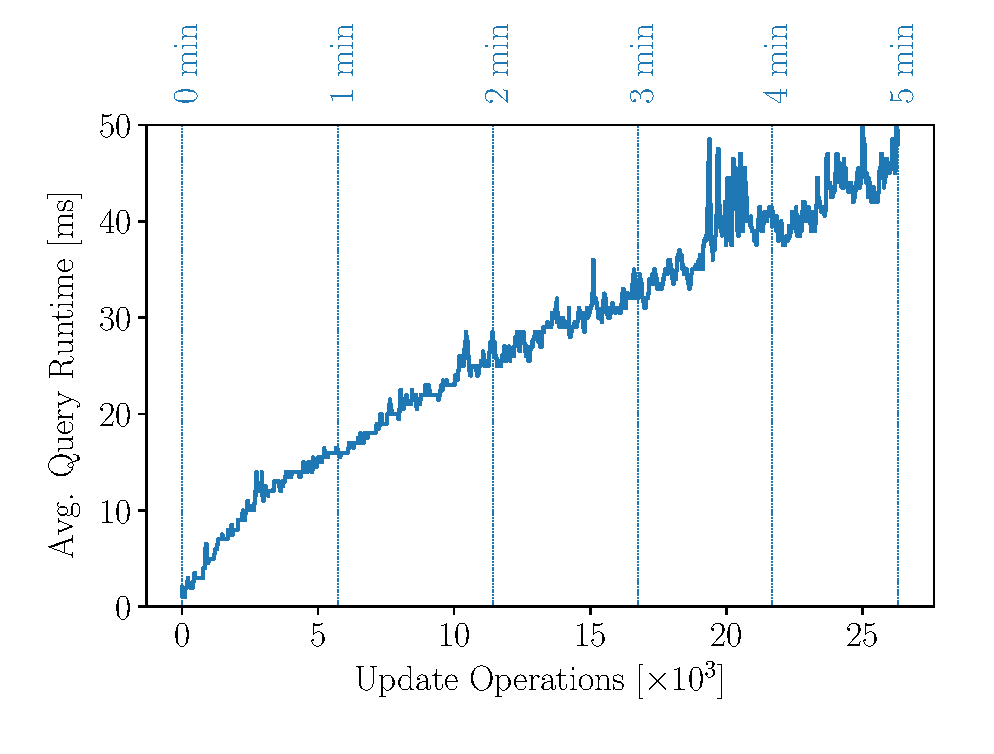
\includegraphics[height=3.8cm]{query_runtime.eps}
        \end{subfigure}
        \begin{subfigure}{0.45\textwidth}
            \centering
            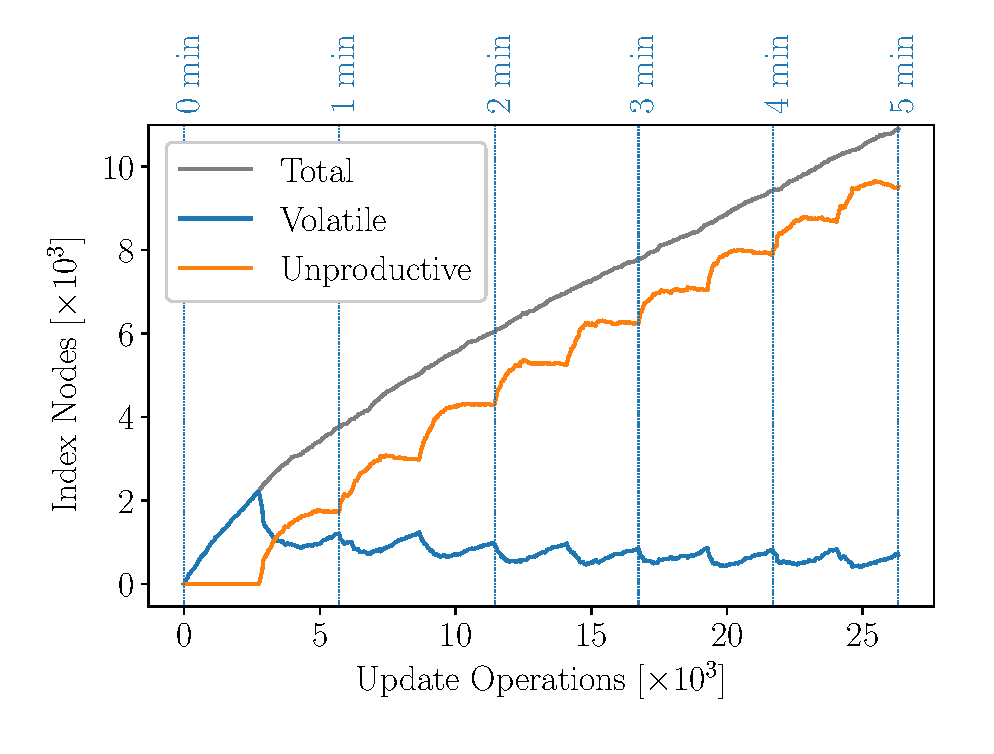
\includegraphics[height=3.8cm]{unprod_nodes.eps}
        \end{subfigure}
    \end{figure}
}
\subsection{Unproductive Nodes}
\frame{
    \centering
    \large
    Volatility threshold $\tau$
}
\frame{
    \frametitle{Volatility threshold $\tau$} 
    \centering
    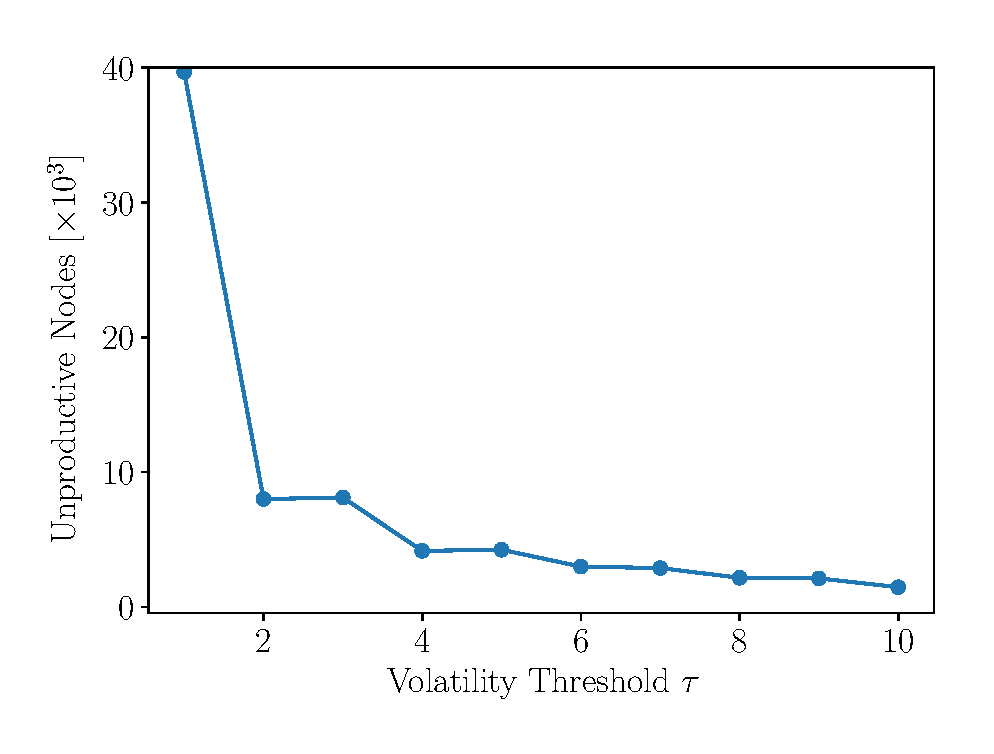
\includegraphics[height=5cm]{tau.eps}
}
\frame{
    \frametitle{Volatility threshold $\tau$} 
    \centering{
        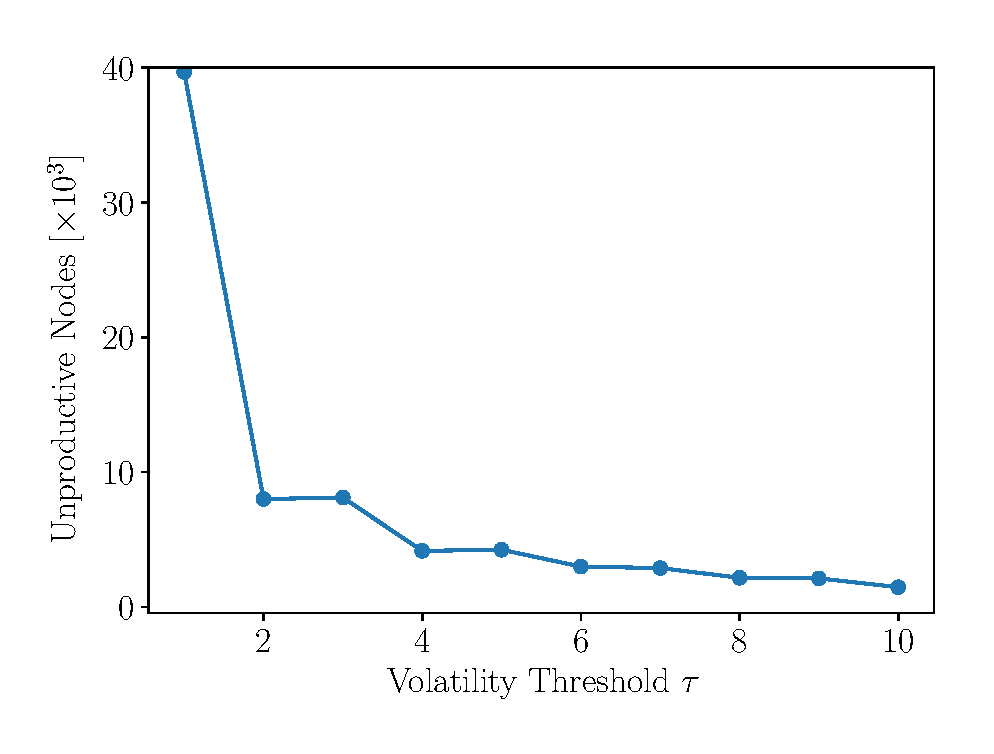
\includegraphics[height=2.5cm]{tau.eps}
    }
    \begin{itemize}
        \item $\tau$ increases $\implies$ nodes are less likely to become volatile
        \item Fewer volatile nodes $\implies$ fewer unproductive nodes
        \item Power law relationship between \#unproductive nodes and $\tau$
    \end{itemize}
}
\frame{
    \centering
    \large
    Workload skew $s$
}
\frame{
    \frametitle{Workload skew $s$}
    \centering
    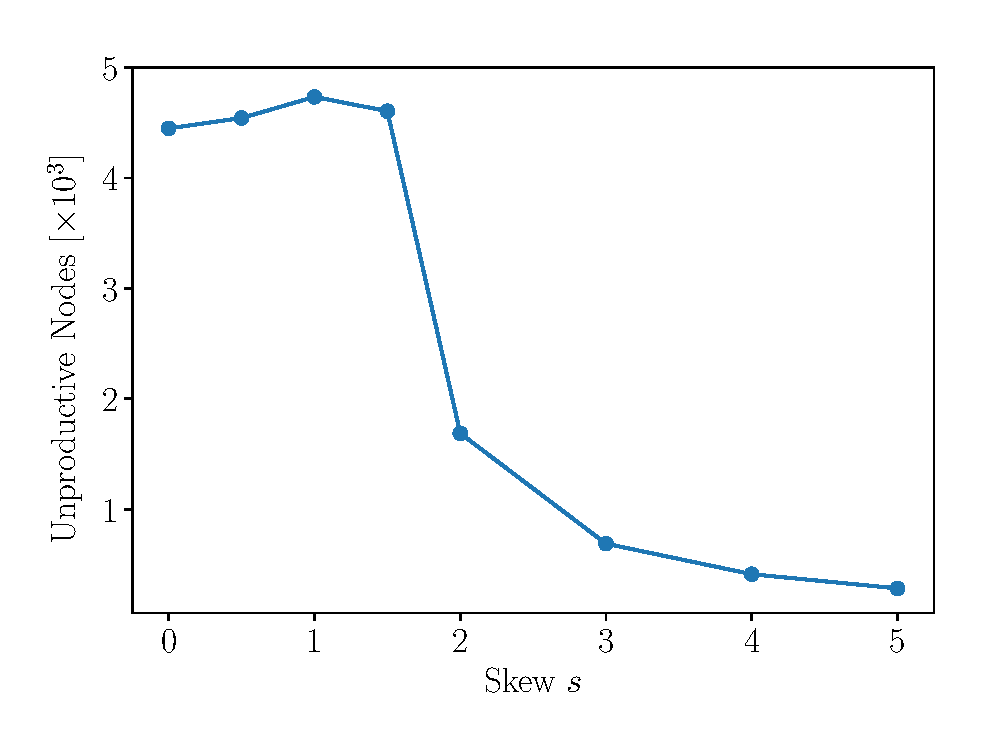
\includegraphics[height=5cm]{skew.eps}
}
\frame{
    \frametitle{Workload skew $s$} 
    \centering{
        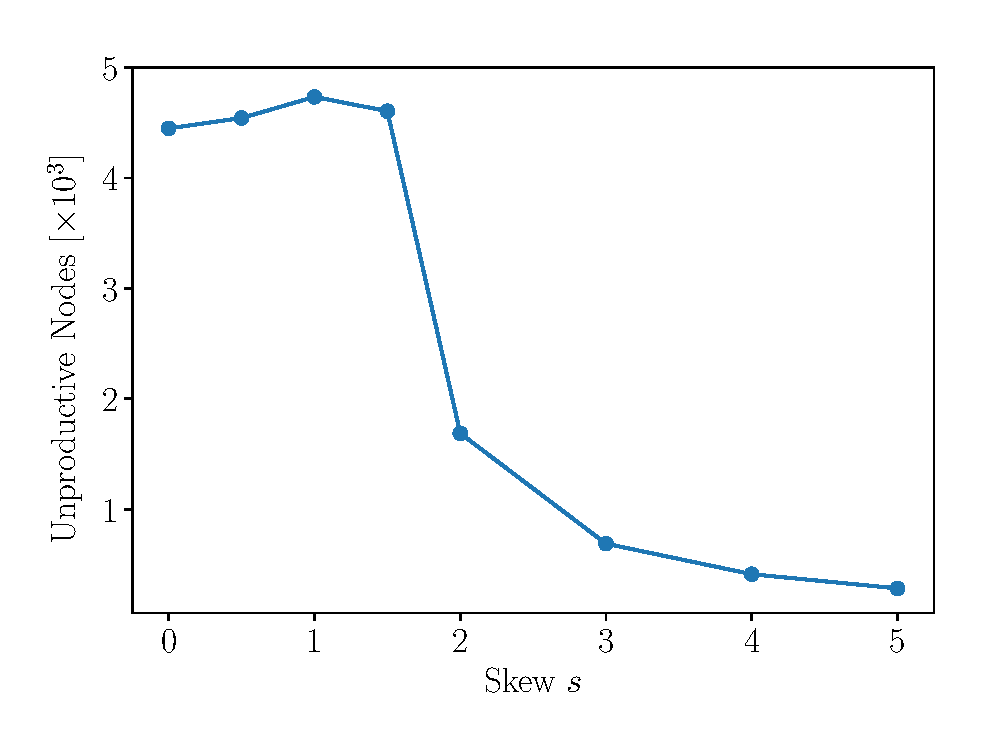
\includegraphics[height=2.5cm]{skew.eps}
    }
    \begin{itemize}
        \item very high $s$ $\implies$ very small hotspot
        \item very small $s$ (uniform) $\implies$ no hotspot
        \item very small/no hotspot $\implies$ nodes are less likely to become volatile
            and later on unproductive
    \end{itemize}
}
\subsection{Periodic Garbage Collection}
\frame{
    \centering
    \large
    Periodic Garbage Collection
}
\frame{
    \frametitle{Periodic GC}
    \begin{figure}
        \begin{subfigure}{0.45\textwidth}
            \centering
            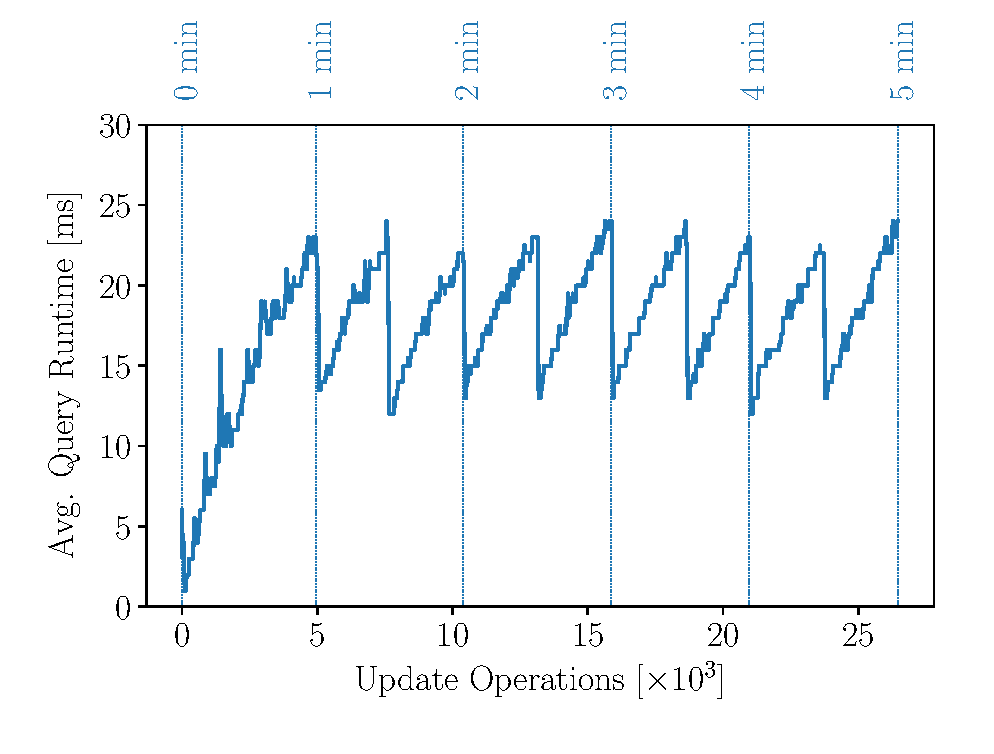
\includegraphics[height=3.8cm]{query_runtime_GC.eps}
        \end{subfigure}
        \begin{subfigure}{0.45\textwidth}
            \centering
            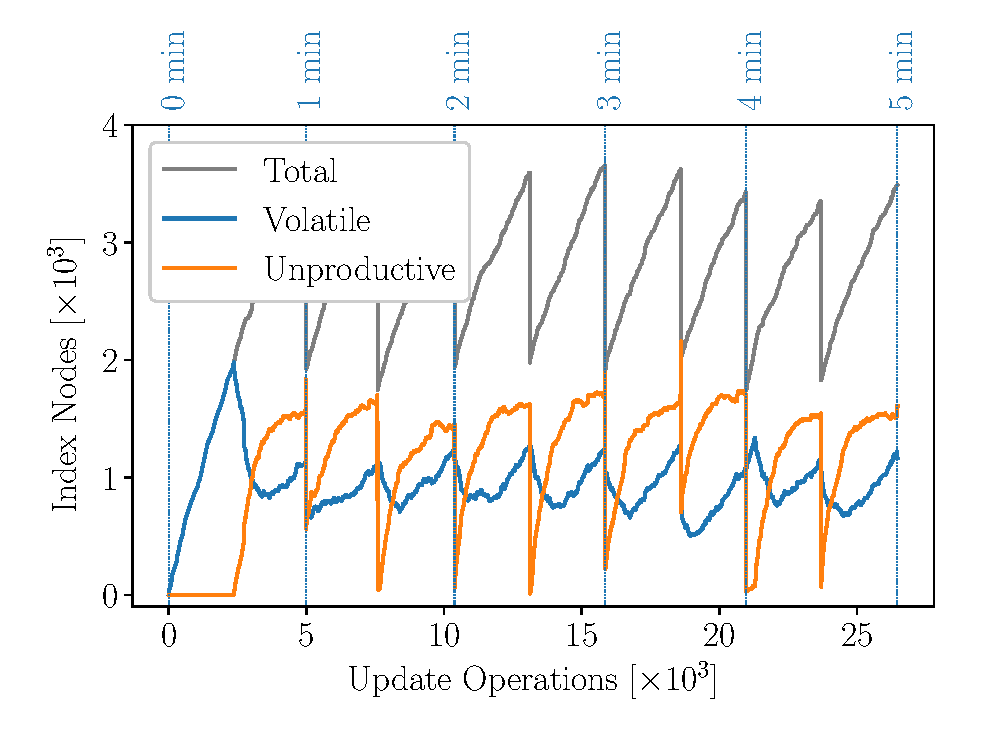
\includegraphics[height=3.8cm]{unprod_nodes_GC.eps}
        \end{subfigure}
    \end{figure}
}
\frame{
    \frametitle{GC period $T$}
    \begin{figure}
        \begin{subfigure}{0.45\textwidth}
            \centering
            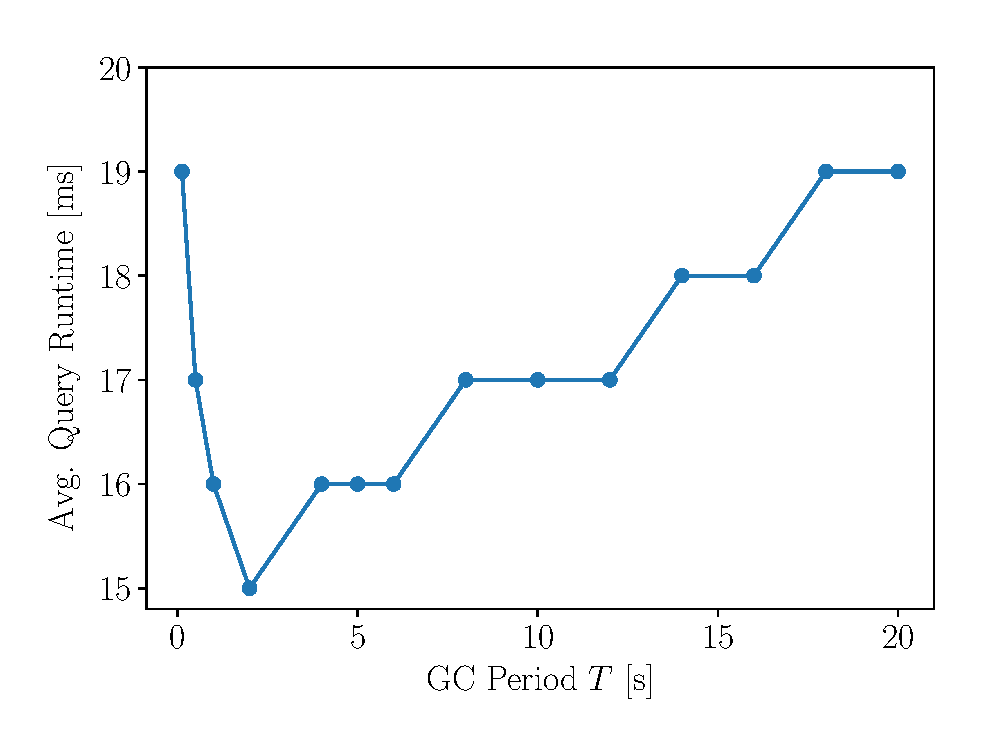
\includegraphics[height=3.8cm]{query_runtime_T.eps}
        \end{subfigure}
        \begin{subfigure}{0.45\textwidth}
            \centering
            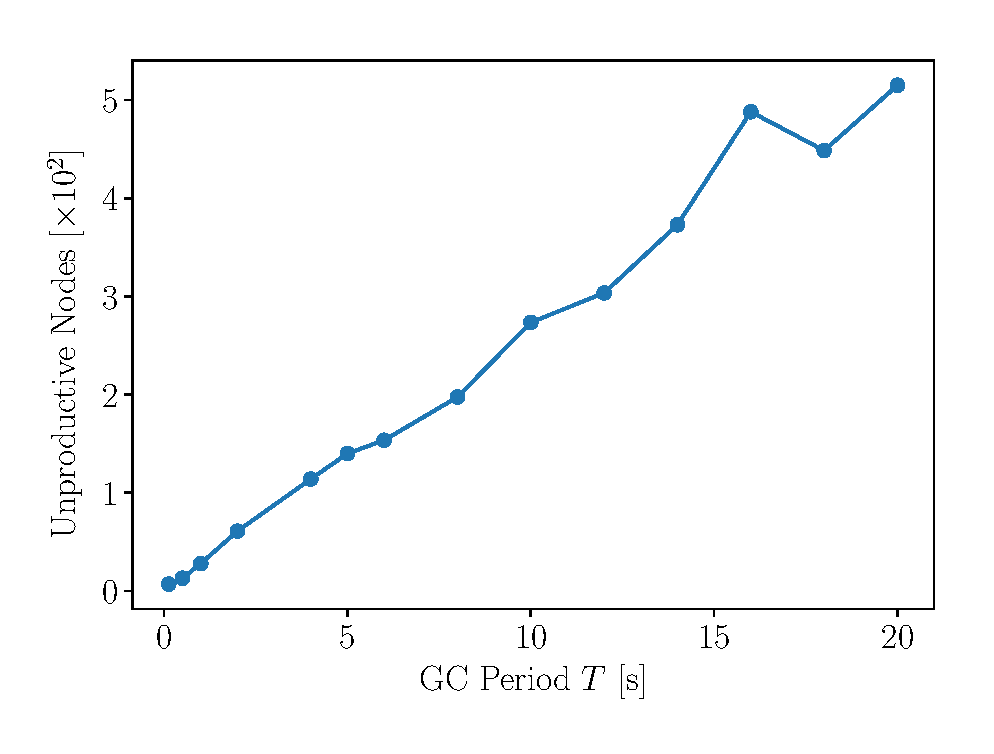
\includegraphics[height=3.8cm]{unprod_nodes_T.eps}
        \end{subfigure}
    \end{figure}

}
\subsection{Query-Time Pruning}
\frame{
    \centering
    \large
   Query-Time Pruning 
}
\frame{
    \frametitle{QTP}
    \begin{figure}
        \begin{subfigure}{0.45\textwidth}
            \centering
            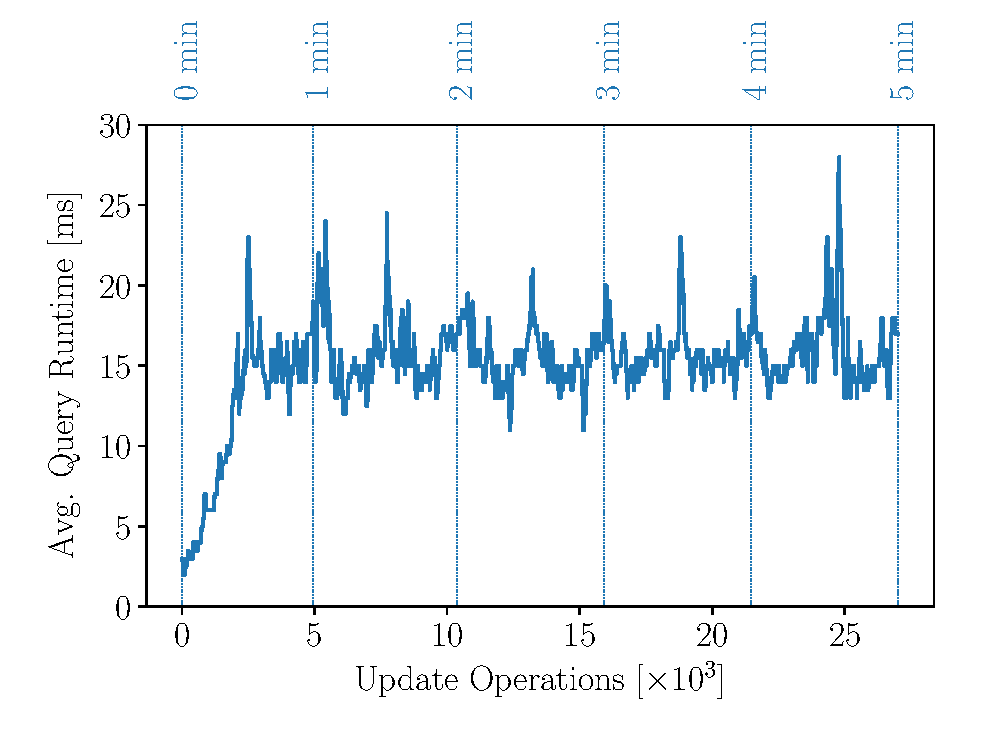
\includegraphics[height=3.8cm]{query_runtime_QTP.eps}
        \end{subfigure}
        \begin{subfigure}{0.45\textwidth}
            \centering
            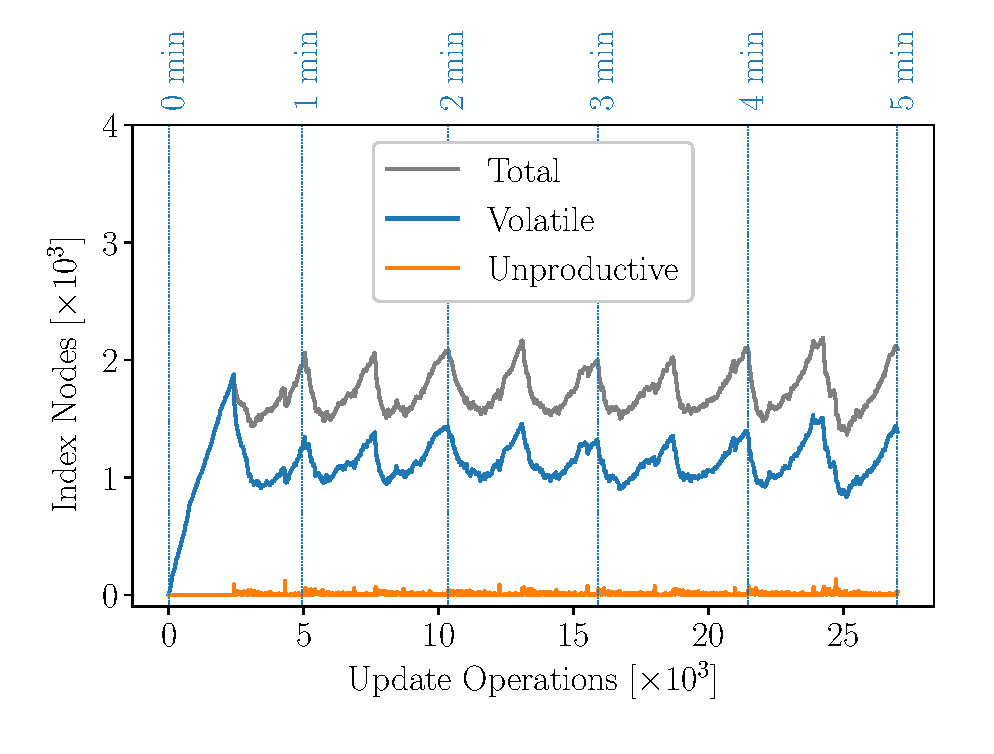
\includegraphics[height=3.8cm]{unprod_nodes_QTP.eps}
        \end{subfigure}
    \end{figure}
}
\frame{
    \frametitle{QTP}
    \begin{figure}[H]
        \centering
        \begin{subfigure}{0.49\linewidth}
            \centering
            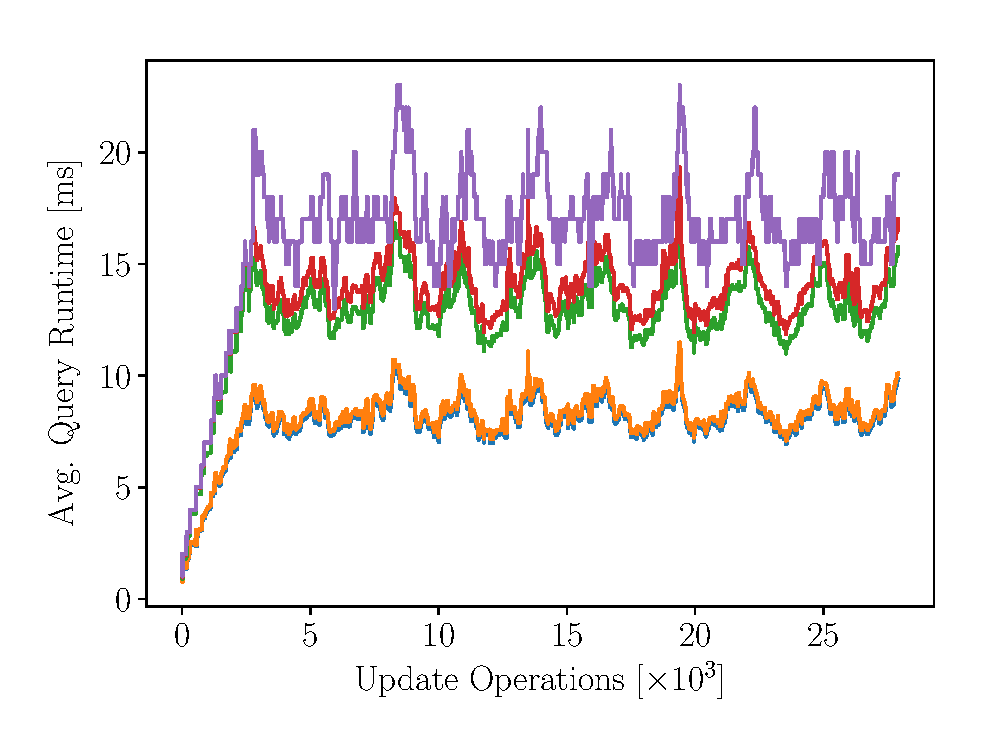
\includegraphics[width=6cm]{qtp_cost.eps}
        \end{subfigure}
        \begin{subfigure}{0.49\linewidth}
            \centering
            \begin{tikzpicture}[scale=0.52]
                \fill[transparent] (-1,0) rectangle (0,5.5);
                \filldraw[color=C0] (0,0) rectangle (1,2.40);
                \filldraw[color=C1] (0,2.40) rectangle (1,2.56);
                \filldraw[color=C2] (0,2.56) rectangle (1,4.01);
                \filldraw[color=C3] (0,4.01) rectangle (1,4.31);
                \filldraw[color=C4] (0,4.31) rectangle (1,5);
                \fill[transparent] (0,5) rectangle (1,5.5);

                \draw[dotted] (0.5,1.3) -- (5.5,0);
                \node[align=left] at (6.7,0) {\footnotesize traversal};

                \draw[dotted] (0.5,2.48) -- (5.5,1.25);
                \node[align=left] at (7.1,1.25) {\footnotesize matching(n)};
                \draw[dotted] (0.5,3.285) -- (5.5,2.5);
                \node[align=left] at (7,2.5) {\footnotesize chd(n) = $\emptyset$};
                \draw[dotted] (0.5,4.16) -- (5.5,4.5);
                \node[align=left] at (6.9,4.5) {\footnotesize volatile(n)};
                \draw[dotted] (0.5,4.66) -- (5.5,5.5);
                \node[align=left] at (6.3,5.5) {\footnotesize write};
                \draw [decorate,decoration={brace,amplitude=10pt,mirror,raise=4pt},yshift=0pt]
                (1.1,2.56) -- (1.1,5.0) node [black,midway,xshift=1.8cm] {\footnotesize
                QTP overhead};
            \end{tikzpicture}
        \end{subfigure}
    \end{figure}
}
\frame{
    \frametitle{QTP}
    \begin{figure}[H]
        \centering
        \begin{subfigure}{0.49\linewidth}
            \begin{algorithm}[H]
                \tiny{
                    \TitleOfAlgo{QueryQTP}
                    \DontPrintSemicolon
                    \KwData{Query $Q(k, v, m)$, where $k$ is a property, $v$ a value and $m$ (=
                        $\texttt{/}\lambda_1\texttt{/}\dots\texttt{/}\lambda_d$) a
                    content node's path.}
                    \KwResult{A set of nodes satisfying $Q(k,v,m)$}
                    $r \longleftarrow \emptyset$\;
                    \For{node $n \in
                        desc(\texttt{/i/k/v/}\lambda_1\texttt{/}\dots\texttt{/}\lambda_d)$ in postorder tree walk}{
                        \uIf{$matching(n)$}{
                            $r \longleftarrow r \cup \{ *n \}$\;
                        }
                        \ElseIf{$chd(n) = \emptyset \land \neg volatile(n)$}{
                            delete node $n$
                        }
                    }
                    \Return{r}\;
                }
            \end{algorithm}
        \end{subfigure}
        \begin{subfigure}{0.49\linewidth}
            \centering
            \begin{tikzpicture}[scale=0.5]
                \fill[transparent] (-1,0) rectangle (0,5.5);
                \filldraw[color=C0] (0,0) rectangle (1,2.40);
                \filldraw[color=C1] (0,2.40) rectangle (1,2.56);
                \filldraw[color=C2] (0,2.56) rectangle (1,4.01);
                \filldraw[color=C3] (0,4.01) rectangle (1,4.31);
                \filldraw[color=C4] (0,4.31) rectangle (1,5);
                \fill[transparent] (0,5) rectangle (1,5.5);

                \draw[dotted] (0.5,1.3) -- (5.5,0);
                \node[align=left] at (6.7,0) {\footnotesize traversal};

                \draw[dotted] (0.5,2.48) -- (5.5,1.25);
                \node[align=left] at (7.1,1.25) {\footnotesize matching(n)};
                \draw[dotted] (0.5,3.285) -- (5.5,2.5);
                \node[align=left] at (7,2.5) {\footnotesize chd(n) = $\emptyset$};
                \draw[dotted] (0.5,4.16) -- (5.5,4.5);
                \node[align=left] at (6.9,4.5) {\footnotesize volatile(n)};
                \draw[dotted] (0.5,4.66) -- (5.5,5.5);
                \node[align=left] at (6.3,5.5) {\footnotesize write};
                \draw [decorate,decoration={brace,amplitude=10pt,mirror,raise=4pt},yshift=0pt]
                (1.1,2.56) -- (1.1,5.0) node [black,midway,xshift=1.8cm] {\footnotesize
                QTP overhead};
            \end{tikzpicture}
        \end{subfigure}
    \end{figure}
}
\subsection{Comparison}
\frame{
    \centering
    \Large
    Periodic GC vs.\ QTP
}
\frame{
    \centering
    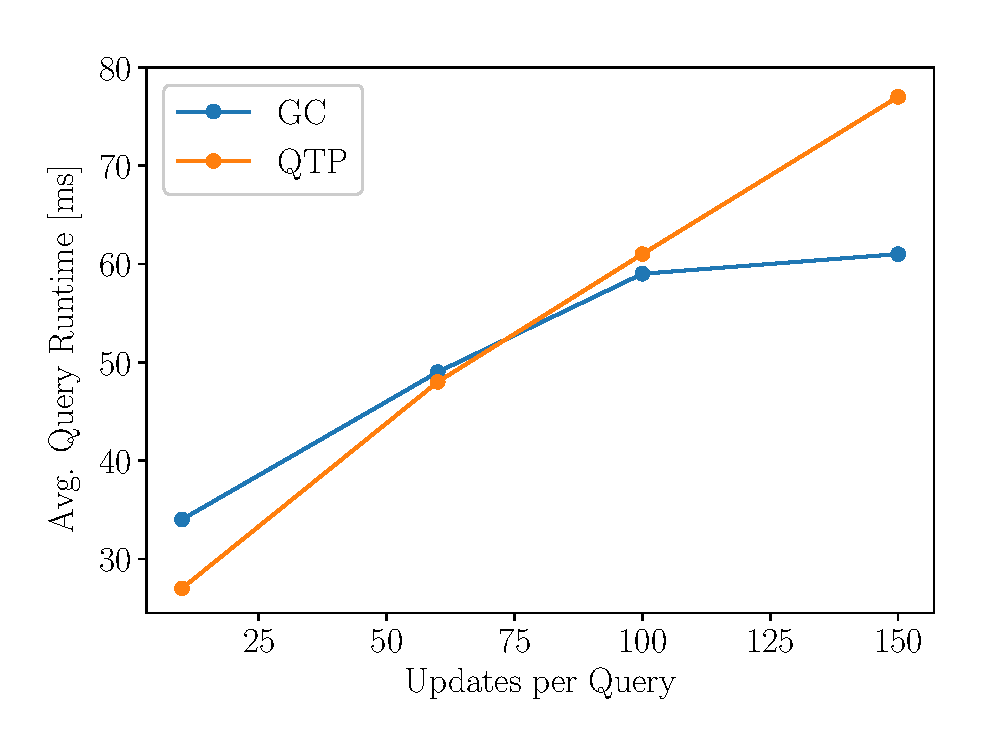
\includegraphics[width=7cm]{gc_vs_qtp.eps}
}
%\subsection{Subsection 1}
%\frame{
    %\frametitle{frame title}
    %\begin{block}{Block title}
        %Block contents
    %\end{block}
    %\begin{itemize}
        %\item item1
        %\item item2
    %\end{itemize}
%}

\section{Conclusion}
\subsection{References}
\frame{
    \frametitle{References}
    \scriptsize
    \bibliography{bib}
}

\end{document}
